\chapter{理論}
\section{AIを用いた楽曲作成}
\subsection{MIDI}
%MIDIとオーディオデータの形式について述べる
パソコンで用いる音楽データには大きく分けて二つある.一つ目はオーディオデータといい波形の情報を記録する形式である.二つ目がMIDIである.\\
 AIによる曲制作では主にMIDIファイルの音楽データを使用する.MIDIファイルは実際の音ではなく音楽の演奏情報(音の高さや長さなど)である.
本研究で用いるAIはこのMIDIファイルの情報を元に学習をする.また入出力の際もこの規格を用いる.\\
 なお,インプットデータはone-hot Vectorで図\ref{fig:インプットデータの仕組み}のようになっている.また,楽曲制作の際に音程を指定する場合は図\ref{fig:MIDIと音階}の数値を指定する.
\begin{figure}[h]
    \begin{screen}
    \begin{center}
        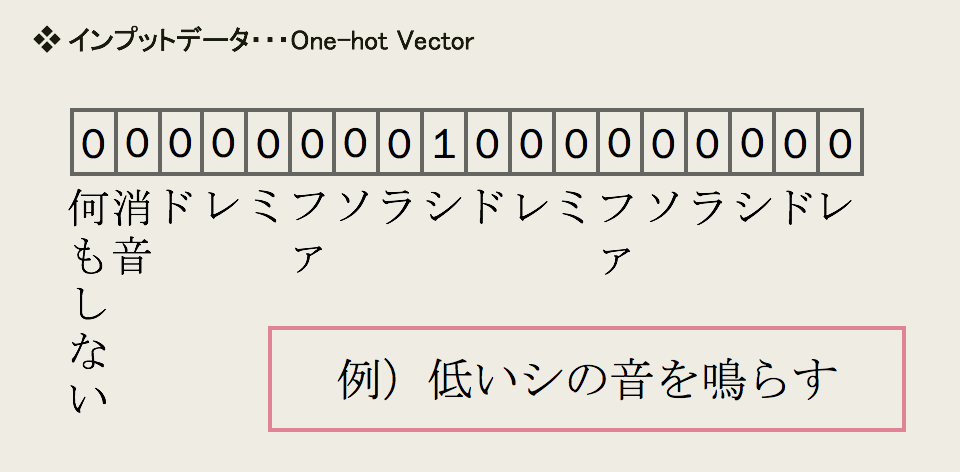
\includegraphics[scale=0.8,clip]{./img/midi1.png}
        \caption{インプットデータの仕組み}
        \label{fig:インプットデータの仕組み}
    \end{center}
    \end{screen}
\end{figure}
\newpage
\begin{figure}[h]
    \begin{screen}
    \begin{center}
        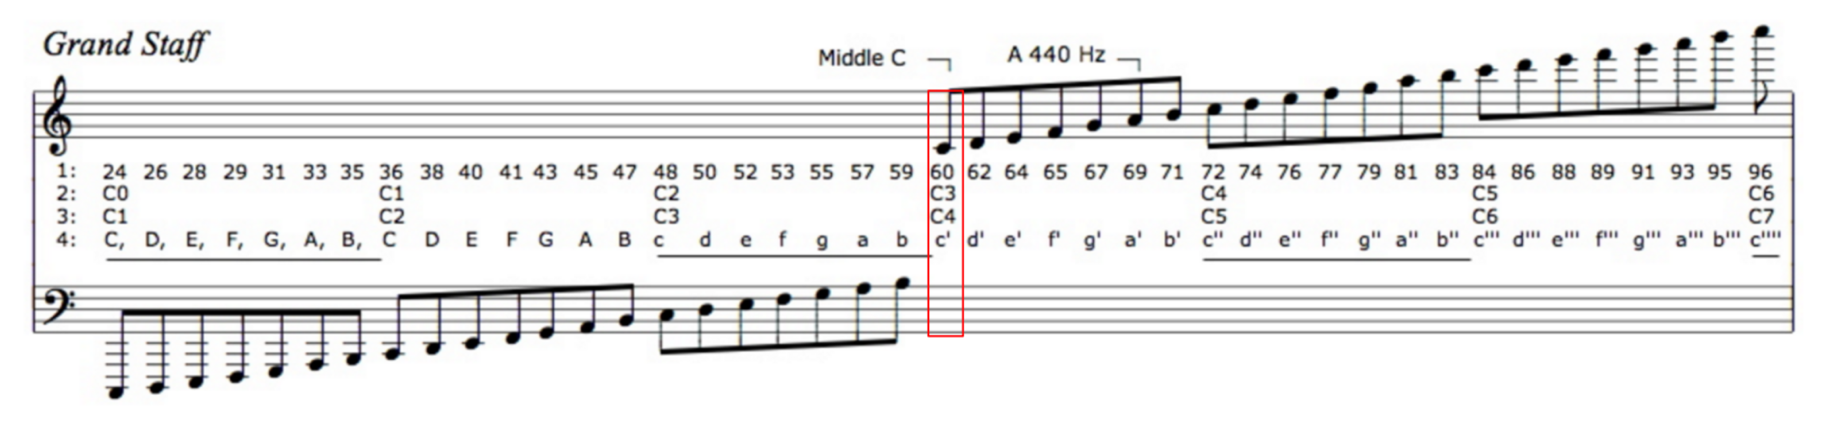
\includegraphics[scale=0.4,clip]{./img/midi2.png}
        \caption{MIDIと音階}
        \label{fig:MIDIと音階}
    \end{center}
    \end{screen}
\end{figure}
%AIを用いた楽曲サービスについて述べてその中でなぜMagendaを選ぶのかを述べる
\subsection{Magenta}
本研究で使用するMagentaは音楽などをTensorFlowを使って機械学習するライブラリであり,Google BrainがGitHub上に公開されているOSSである.これを図\ref{fig:GitHub上に公開されているMagenta}に示す.\\
 Magentaではまず学習させたい音楽のMIDIデータをNoteSequence(magentaが扱うファイル形式)とよばれるデータフォーマットに変更する.それを学習用データセットと評価用データセットに変換したあと学習を行う.
このとき,一度に学習させるデータの数,学習を行う回数,ノード数を設定する.これをパッケージ化し,MIDIファイルとして新たに楽曲を生成するという流れである.これを図\ref{fig:magentaによるMIDI音楽データ生成までのプロセス}に示す.
\begin{figure}[h]
    \begin{screen}
    \begin{center}
        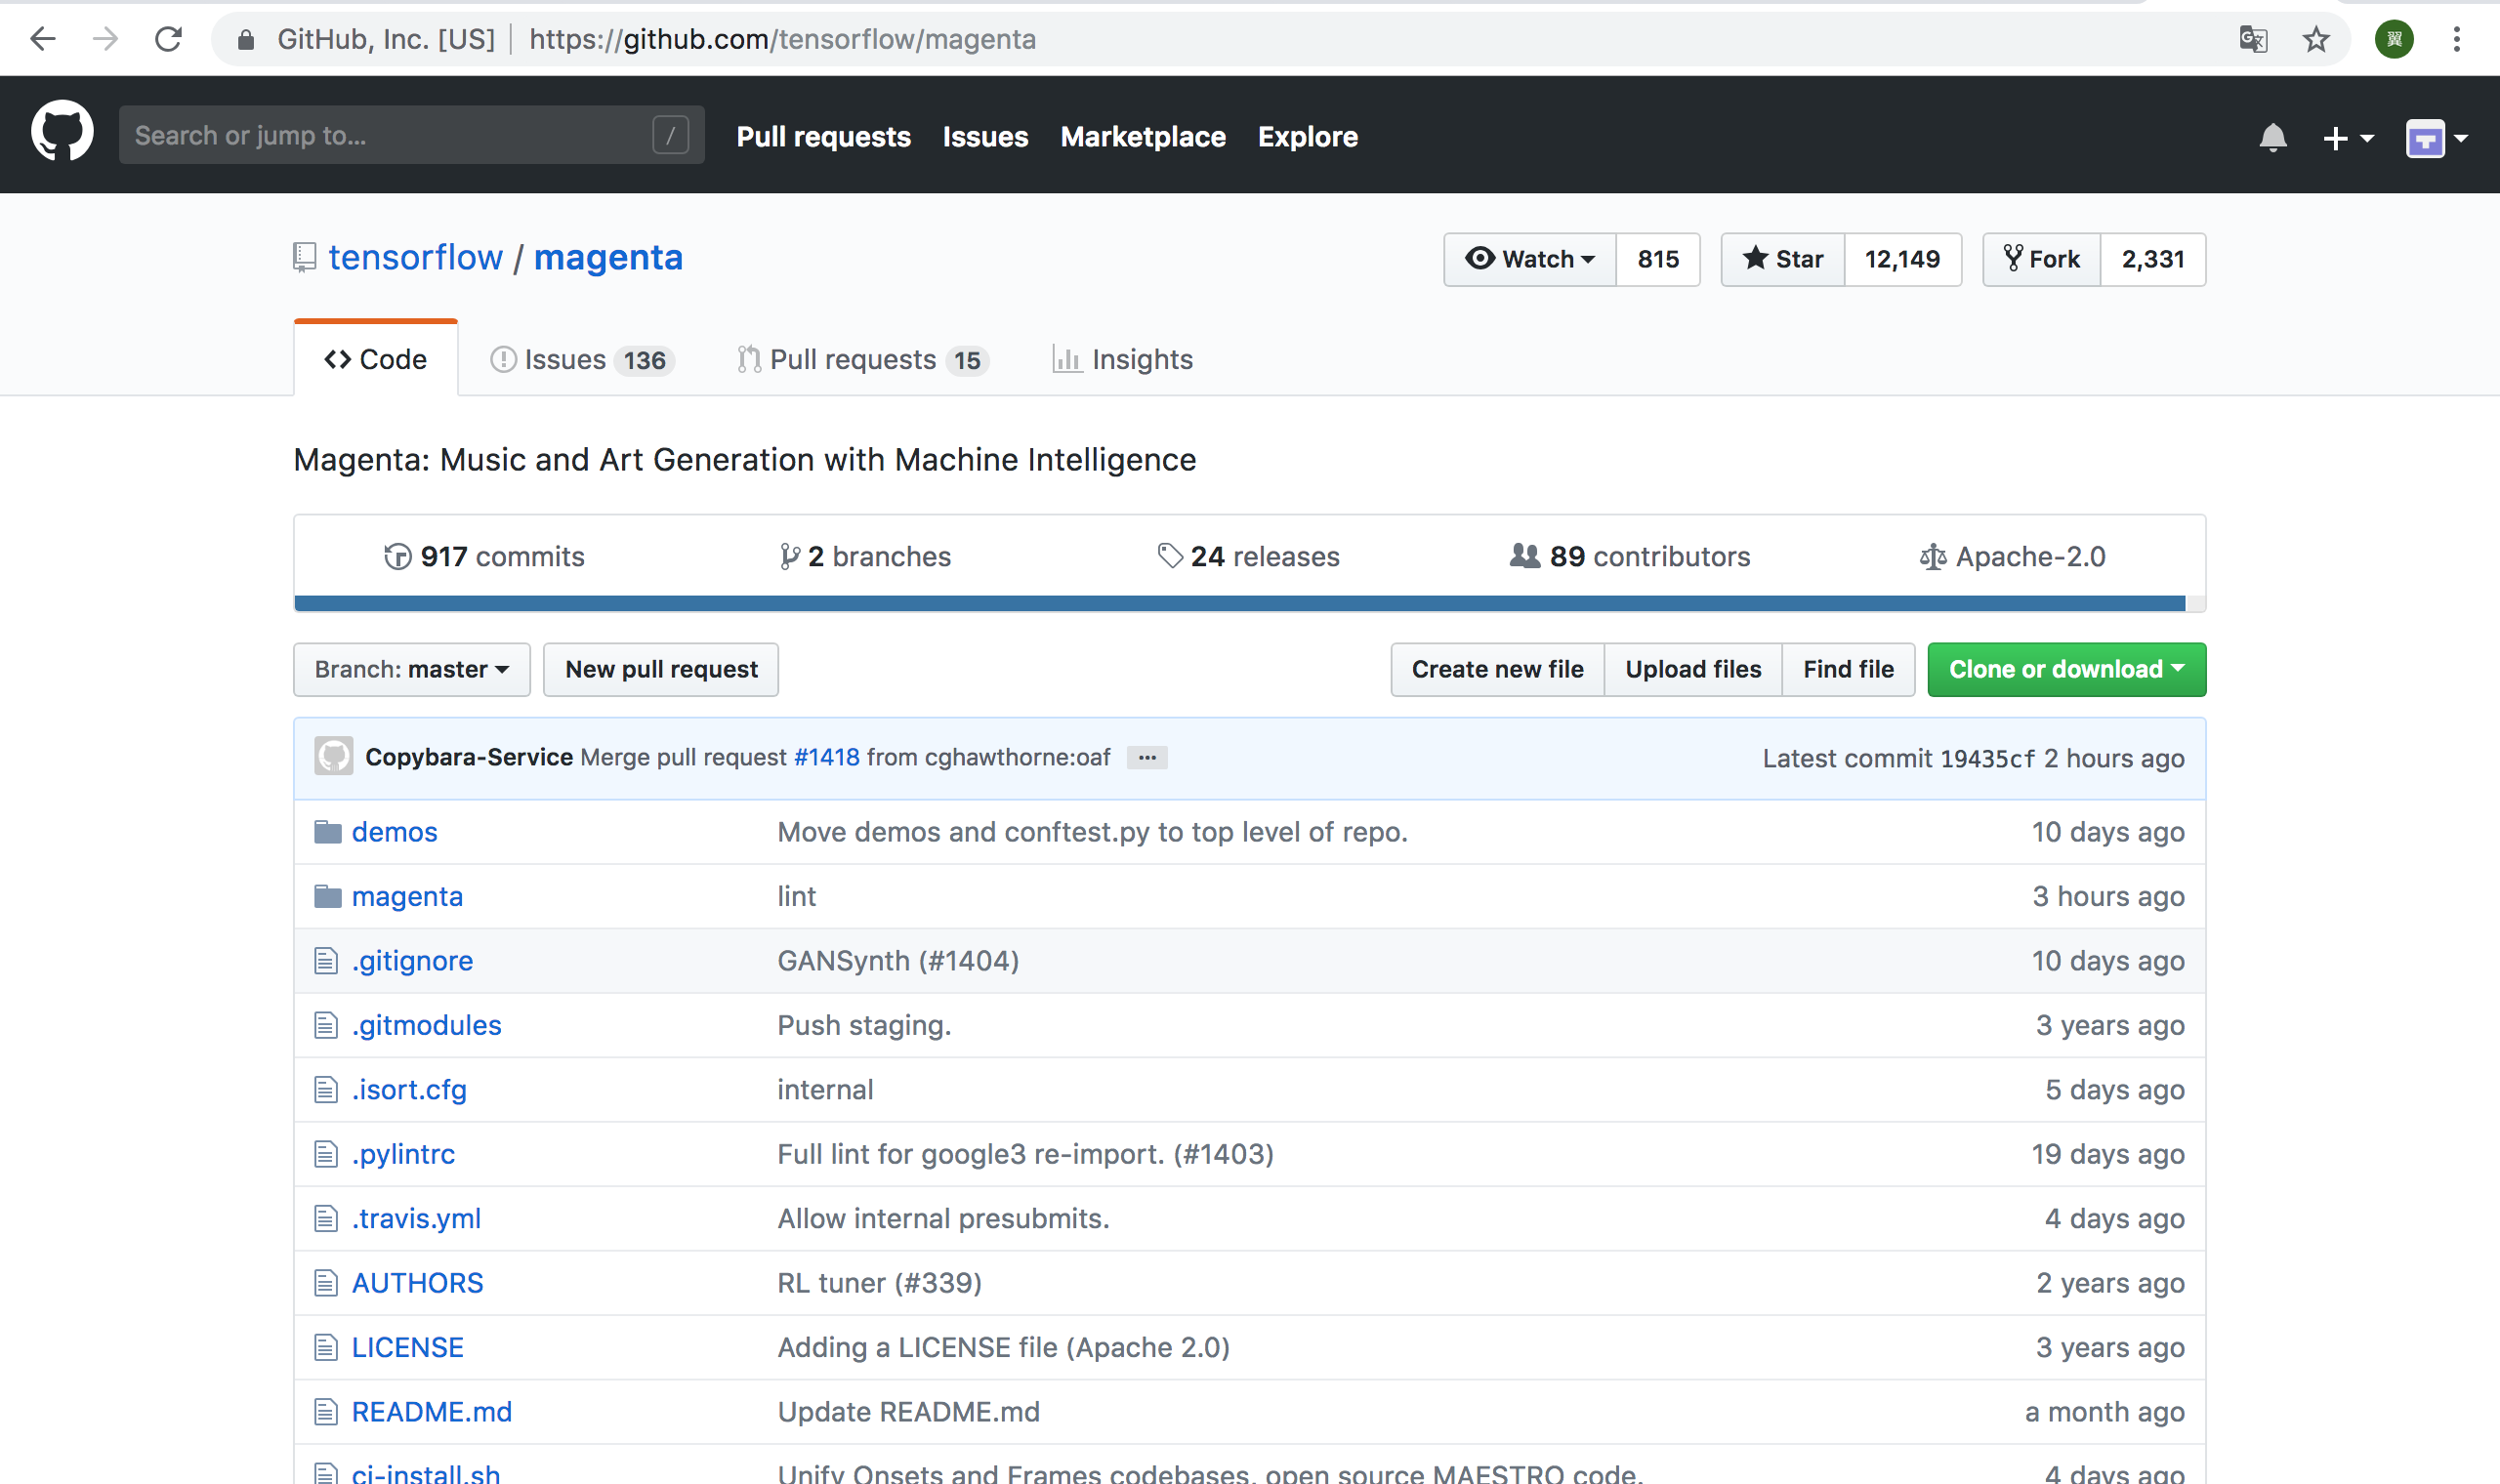
\includegraphics[scale=0.3, clip]{./img/magentagithub.png}
        \caption{GitHub上に公開されているMagenta}
        \label{fig:GitHub上に公開されているMagenta}
    \end{center}
    \end{screen}
\end{figure}
\newpage
\begin{figure}[h]
    \begin{screen}
    \begin{center}
        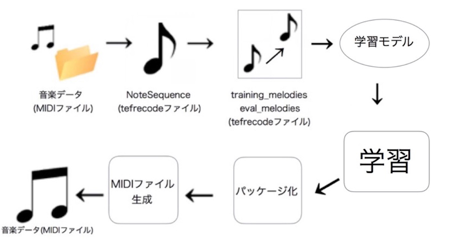
\includegraphics[scale=1.7, clip]{./img/magenta_usestep.png}
        \caption{magentaによるMIDI音楽データ生成までのプロセス}
        \label{fig:magentaによるMIDI音楽データ生成までのプロセス}
    \end{center}
    \end{screen}
\end{figure}
\newpage
\section{機械学習に適した開発環境について}
Tensolflowのランタイムとして以下のシステムがサポートされている.
\begin{enumerate}
    \renewcommand{\labelenumi}{(\arabic{enumi})}
    \item Ubuntu 16.04以降
    \item macOS 10.12.6(Sierra)以降(GPUサポートなし)
    \item Windows7 以降
    \item Raspbian 9.0以降
\end{enumerate}
 また,GPUを用いて学習を行う時にはtensolflow-gpuというパッケージが必要となり,導入には以下のドライバやライブラリが必要である.
\begin{enumerate}
    \renewcommand{\labelenumi}{(\arabic{enumi})}
    \item CUDA Toolkit (tensolflowはCUDA9.0をサポート)
    \item CUPTI (CUDA Toolkitに付随)
    \item NVIDEAGPUドライバ(CUDA9.0には384.x以上が必要)
    \item cuDNN SDK
\end{enumerate}
 Windows10の環境ではリリースされているCUDAのバージョンは10のみであり,Tensolflowのサポートを外れてしまう.
そのため,CUDAv9がインストール可能なUbuntuを用いることとし,システムの開発環境を表\ref{tab:開発環境}に示す.
\begin{table}[h]
\begin{center}
\caption{開発環境}
\label{tab:開発環境}
\begin{tabular}{|c|p{20zw}|}
\hline
    OS & Ubuntu 16.04 LTS\\
    \hline
    CPU & Intel Core i3 8100\\
    \hline
    メモリ & 8GB\\
    \hline
    GPU & GeForce GTX 1060\\
    \hline
    CUDA & CUDA(9),cuDNN(7.4.2)\\
    \hline
    ライブラリ & TensorFlow(1.12.0),magenta(0.5.0)\\
    \hline
\end{tabular}
\end{center}
\end{table}\\
\newpage
\subsection{CUDA}
CUDAは,NVIDIAが開発しているGPU上でプログラミングをするためのソフトウェアプラットフォームである.
含まれるものとしては,CUDAを実行形式に変えるコンパイラや,それをサポートするSDK,ライブラリ,デバッグツール群である.
CUDAを導入することによって,プログラムを複数のプロセッサで動かすだけでなく,無駄なく並列化することができる.